\chapter{Properties of Euclidean Voronoi Diagrams}

% % % % % % % % % % % % % % % % % % % % % % % % % % % % % % % % % % % %
%
% Definition
%
% % % % % % % % % % % % % % % % % % % % % % % % % % % % % % % % % % % % 
In this chapter we will consider Voronoi diagrams for the $L^2$ norm, also known as the Euclidean norm. The norm is given by
\[
    \norm{(x, y)}_2 = \sqrt{x^2 + y^2},
\]
for all $x, y \in \R$. Here is the example diagram with this norm from earlier:
\begin{figure}[H]
    \centering
    \subfloat{
      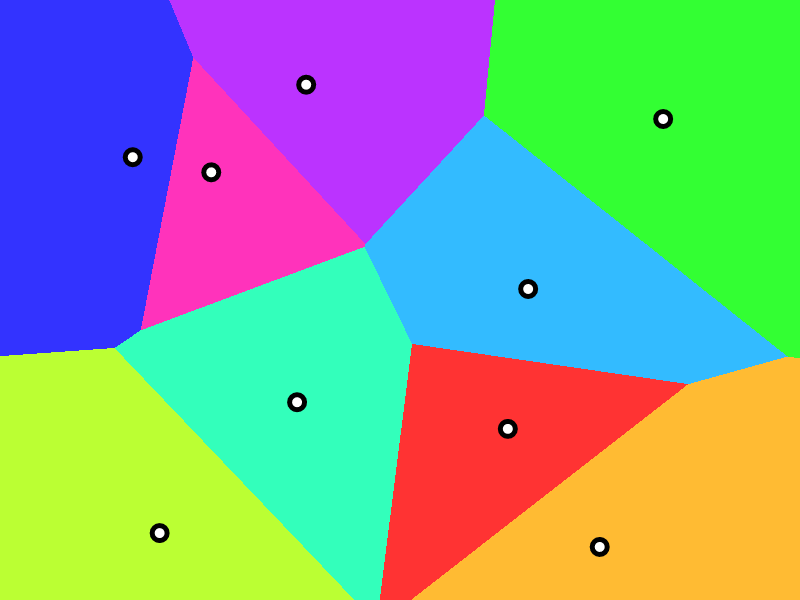
\includegraphics[scale=0.21]{naive-voronoi-L2}
    }
    \subfloat{
      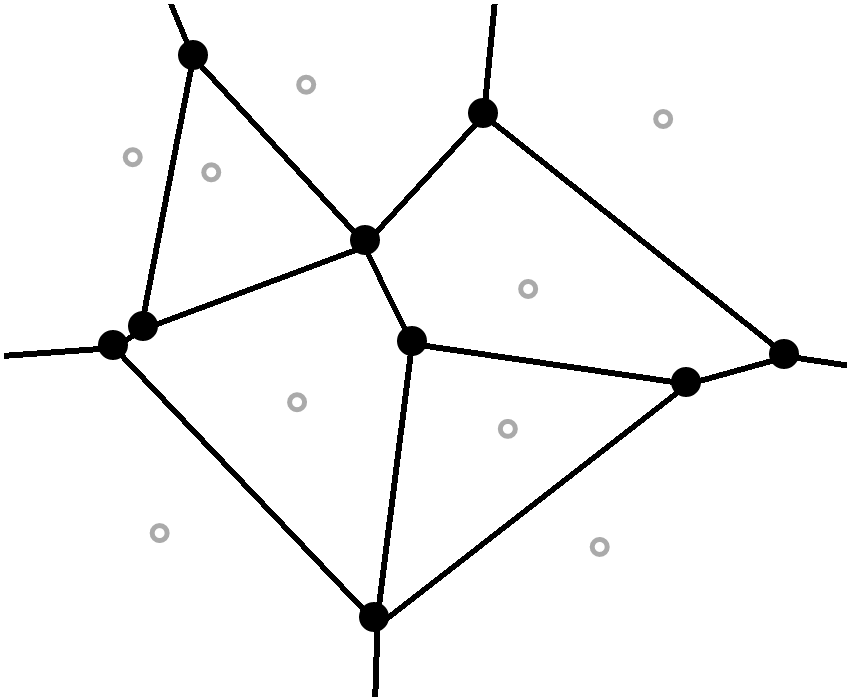
\includegraphics[scale=0.18]{naive-voronoi-graph-L2}
    }
\end{figure}
We note that the diagram consists of straight lines, rays and line segments. In the following sections we will describe the shape of the diagram in detail.

% % % % % % % % % % % % % % % % % % % % % % % % % % % % % % % % % % % %
%
% Preliminary definitions: Bisector, halfplane, Voronoi cells
%
% % % % % % % % % % % % % % % % % % % % % % % % % % % % % % % % % % % % 

\section{Bisectors, halfplanes and Voronoi cells}
From linear algebra we know that $\norm{v}_2 = \sqrt{\ip{v}{v}}$, where $\ip{\,\cdot\,}{\,\cdot\,}$ is the usual dot product on $\R^2$. Given two points $p, q \in \R^2$ then the \textbf{bisector} of $p$ and $q$ is denoted by $\bi(p, q) \subset \R^2$ and denotes the set of points on a line $\ell$ which passes through the midpoint of $p$ and $q$ and is orthogonal (w.r.t. $\ip{\,\cdot\,}{\,\cdot\,}$) to the vector $p - q$.
\[
    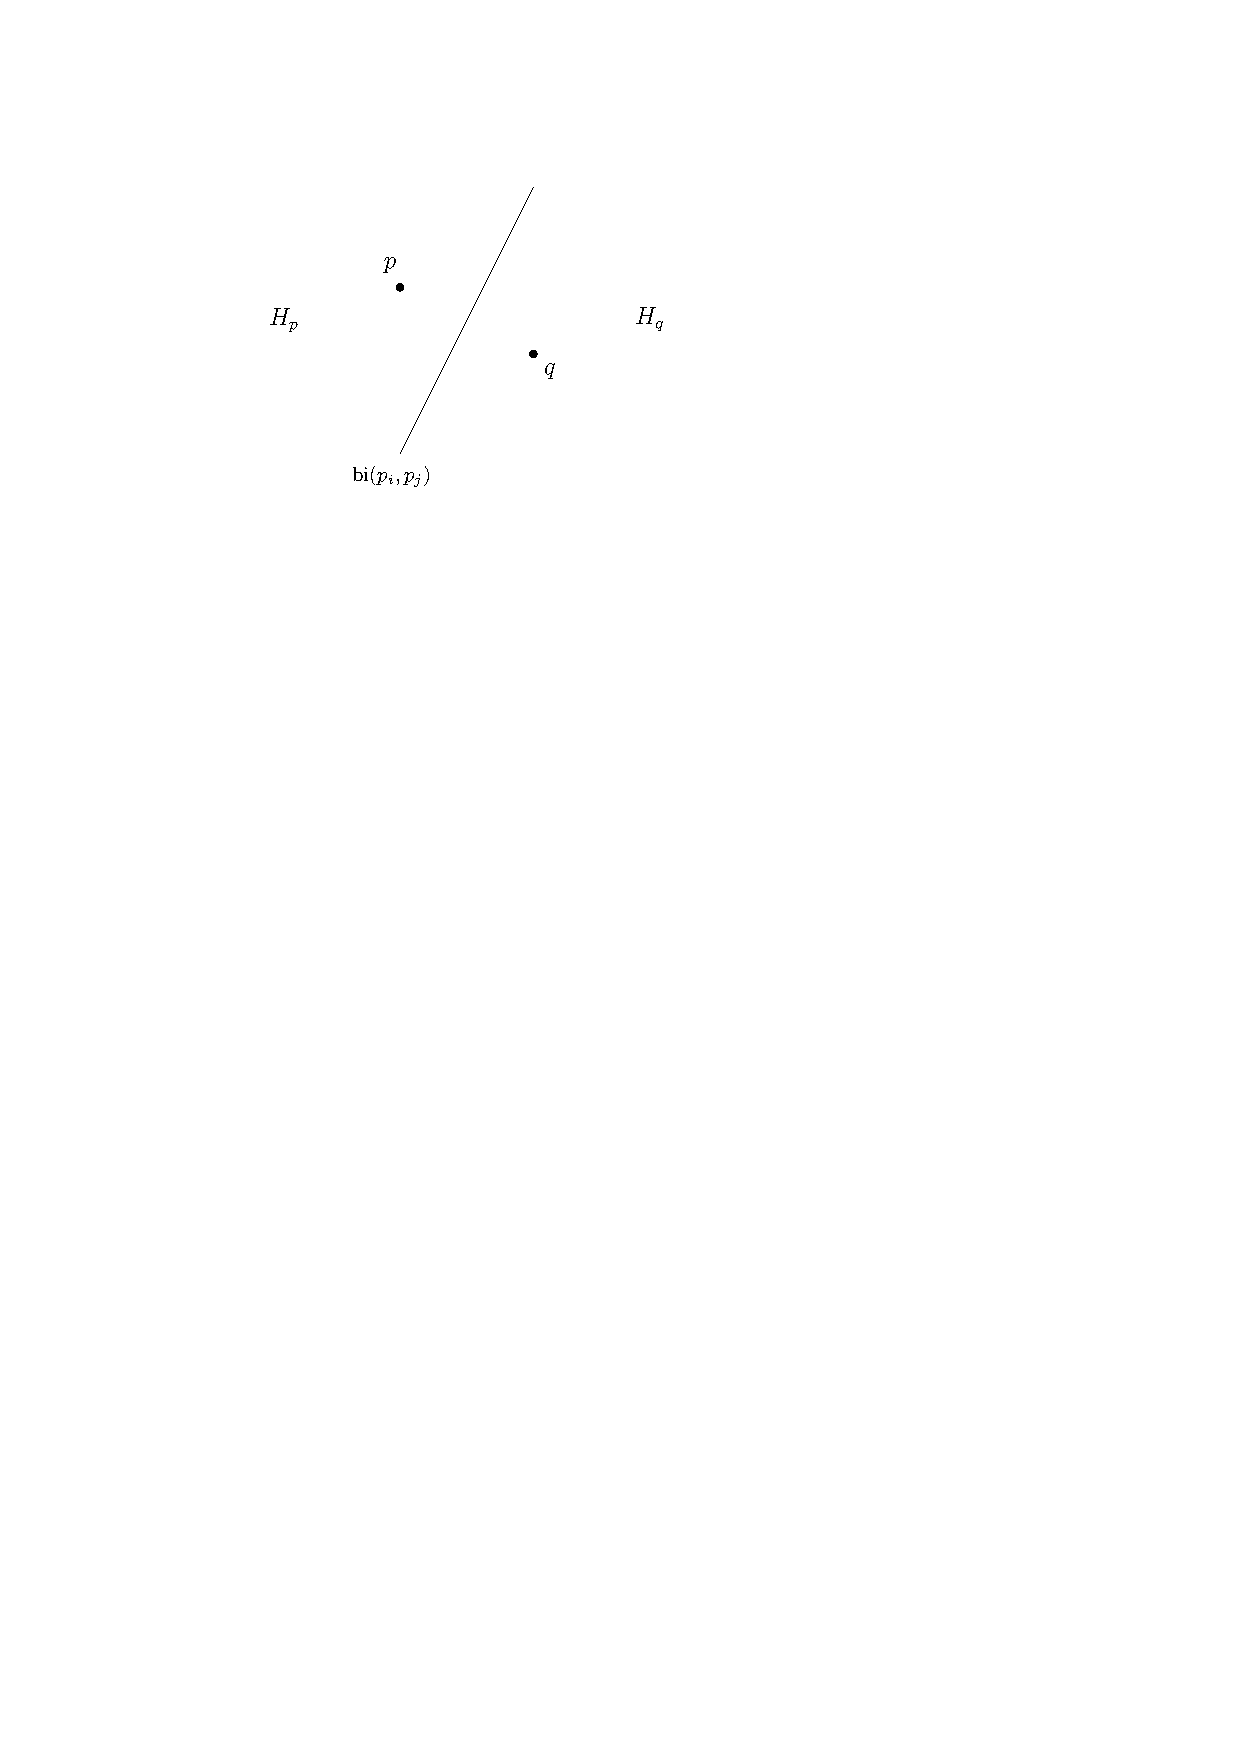
\includegraphics[scale=0.8]{bisector} %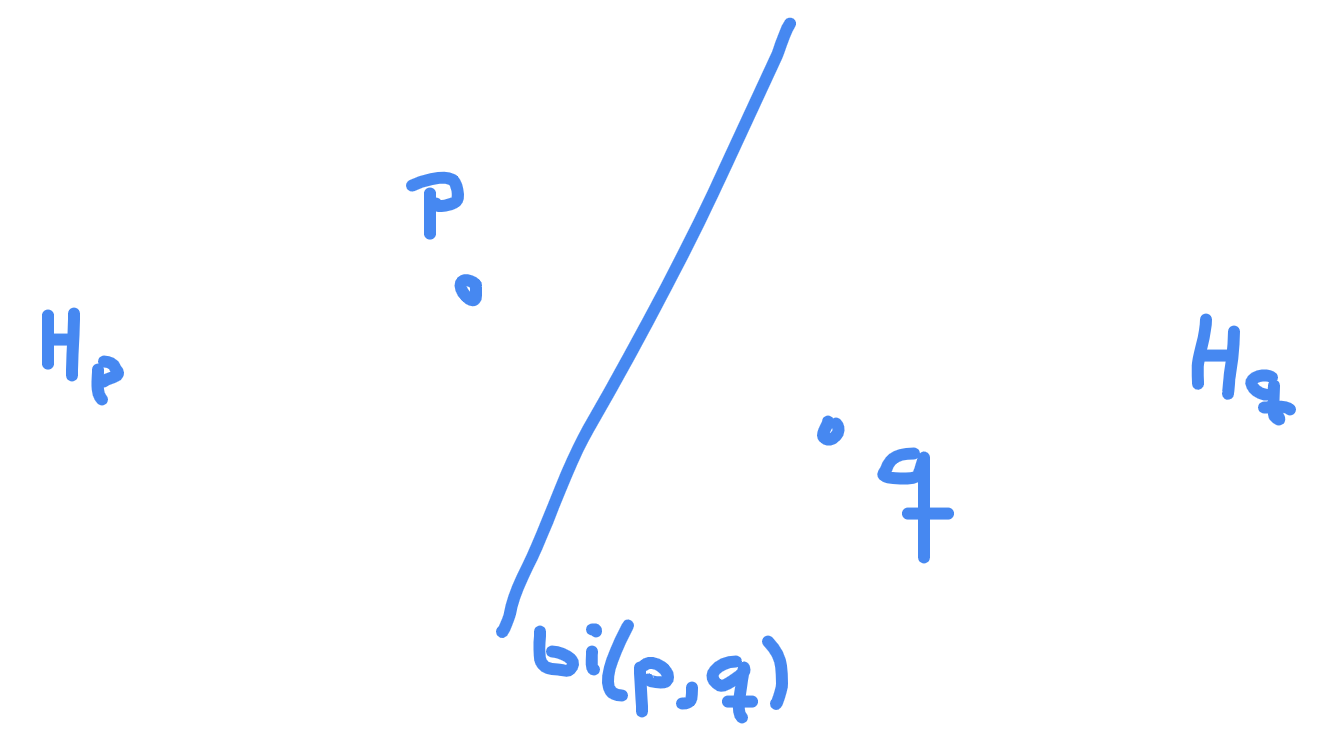
\includegraphics[scale=0.22]{temp-fig-2}
\]
A bisector $\bi(p, q)$ splits the plane into two \textbf{half-planes} $H_p$ and $H_q$ such that $p \in H_p$ and $q \in H_q$. We define $h(p, q)$ to be the open half-plane which contains $p$, that is the interior of $H_p$. So we have that
\[
    \R^2 = h(p, q) \cup \bi(p, q) \cup h(q, p).
\]
\begin{prop} \label{prop:hyperplaneinclusionproperty}
$r \in h(p, q)$ if and only if $\dist(r, p) < \dist(r, q)$.
\end{prop}
\begin{proof}
Let $r \in h(p, q)$ and let $s$ be the projection of $r$ onto the line segment $\overline{pq}$.
\[
    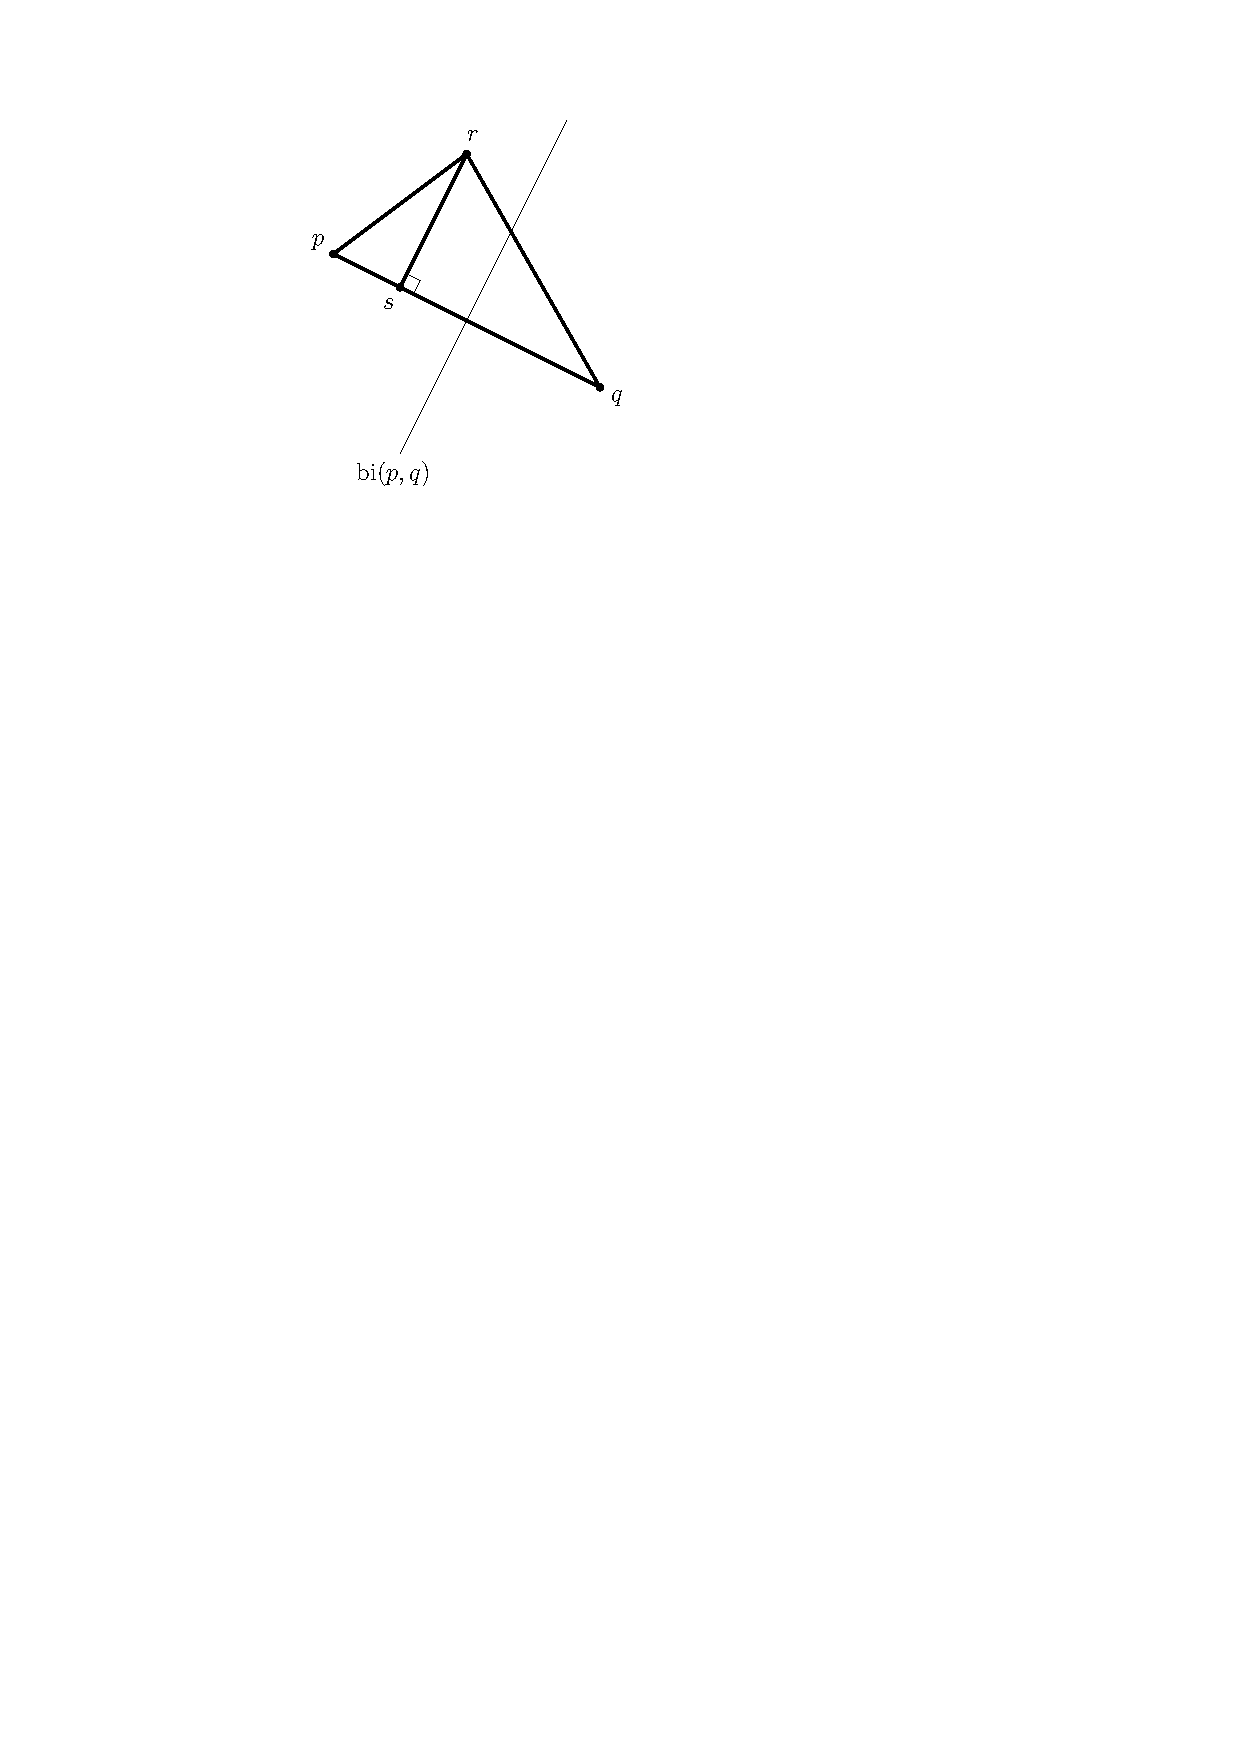
\includegraphics[scale=0.8]{halfplane_containment} %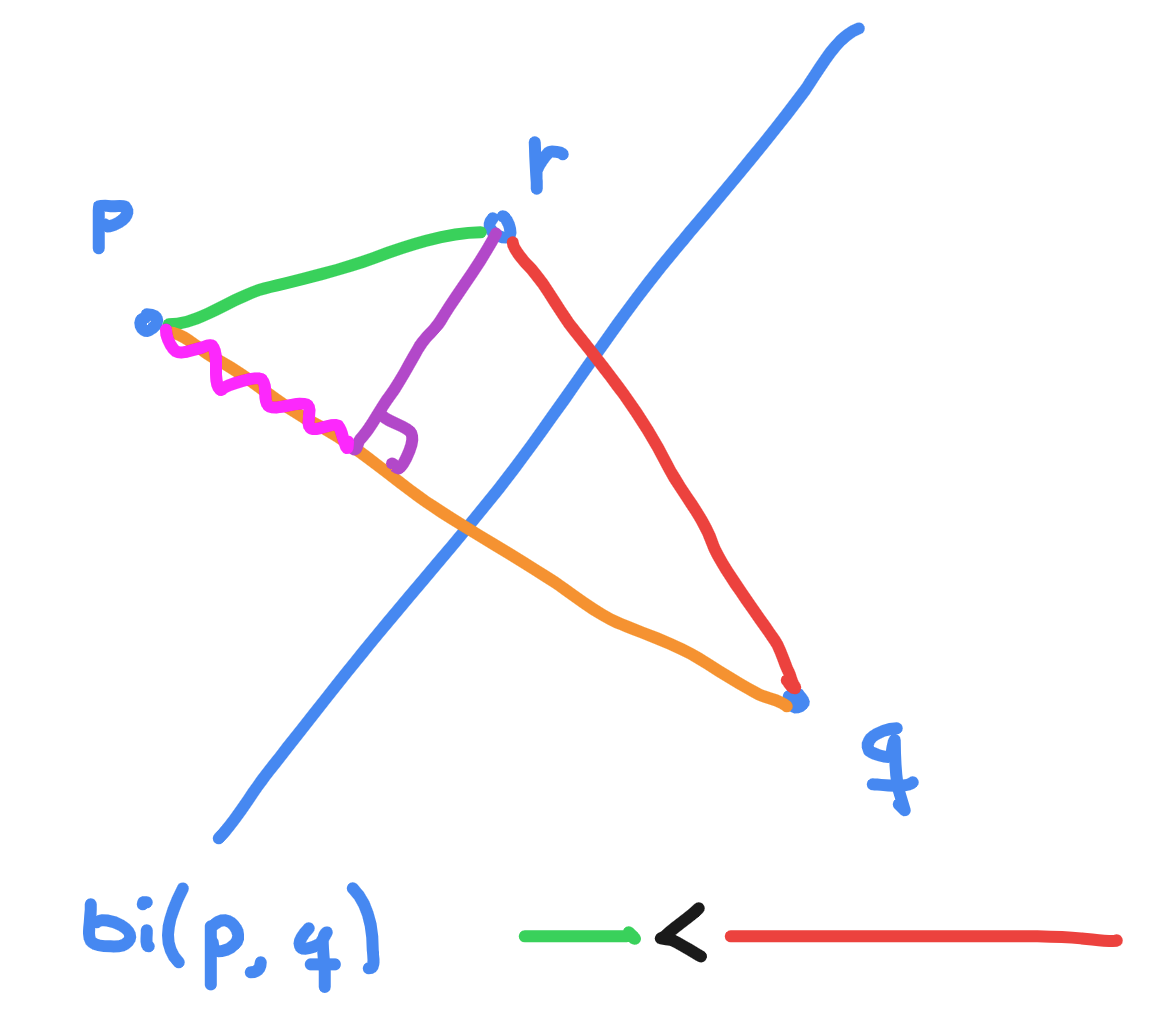
\includegraphics[scale=0.25]{temp-fig-1}
\]
The Pythagorean theorem and the fact that $\overline{ps}$ is shorter than $\overline{sq}$ then gives us
\begin{align*}
    \norm{p - r}^2 &= \norm{p - s}^2 + \norm{s - r}^2 \\
    &< \norm{q - s}^2 + \norm{s - r}^2 \\
    &= \norm{q - r}^2,
\end{align*}
which gives us that $\dist(r, p) < \dist(r, q)$. The other direction is symmetrical.

%\todo{Formalize} Proof sketch: We want to project $r$ onto the orange line. As long as $r \in H_p$ then the squiggly pink segment is shorter than the orange segment, which will make the green segment shorter than the red segment (which is what we want to show).
\end{proof}

\begin{cor} \label{prop:cellsareintersectionsofhalfplanes}
For every Voronoi cell we have
\[
    \mathcal{V}(p_i) = \bigcap_{\substack{1 \leq j \leq n \\ j \ne i}} h(p_i, p_j).
\]
\end{cor}
\begin{proof}
``$\subset$'': Let $r \in \mathcal{V}(p_i)$. Then $\dist(r, p_i) < \dist(r, p_j)$ for all $i \ne j$. Prop \ref{prop:hyperplaneinclusionproperty} then gives us that this is equivalent to $r \in h(p_i, p_j)$ for all $i \ne j$.

``$\supset$'': This argument is symmetrical to the above argument.
\end{proof}
A Voronoi cell is thus the intersection of convex sets and is therefore convex. We conclude that the Voronoi cells are open and convex (possibly unbounded) polygons with at most $n - 1$ vertices and $n - 1$ edges. \\

\section{Shape of the entire diagram}
We now look at the shape of the entire Voronoi diagram. From Corollary \ref{prop:cellsareintersectionsofhalfplanes} it follows that the edges of $\VorG(P)$ are made up of parts of straight lines, namely the bisectors between different points of $P$. We now classify these based on the structure of the points in $P$:
\begin{thm} \label{prop:structureofentirevoronoidiagram}
If the points in $P$ are collinear then $\VorG(P)$ consists of $n - 1$ parallel lines. Otherwise, $\VorG(P)$ is connected and its edges are either segments or half-lines.
\end{thm}
\begin{proof}
Assume that the points in $P$ are collinear. By applying an isometry to $P$, we may assume without loss of generality that the points of $P$ lie on the $x$-axis:
\[
    P = \curly{(x_1, 0), (x_2, 0), \ldots, (x_n, 0)},
\]
where we assume that $x_1 < x_2 < \cdots < x_n$ by rearranging the points if necessary. See the proof of Theorem \ref{thm:voronoicansort} for a visualization of $\Vor(P)$. By definition, we have that $p \in \VorG(P)$ if and only if $p \not\in \mathcal{V}(x_i, 0)$ for all $i$. Let $(x, y) \in \R^2$ such that $x_i < x < x_{i+1}$. Then $(x, y) \in \VorG(P)$ if
\[
    \dist((x, y), (x_i, 0)) = \dist((x, y), (x_{i+1}, 0)).
\]
If furthermore $(x, y) \in \VorG(P)$ then we get
\begin{align*}
    &\norm{(x, y) - (x_i, 0)} = \norm{(x, y) - (x_{i+1}, 0)} \\
    \iff &\sqrt{(x - x_i)^2 + y^2} = \sqrt{(x - x_{i+1})^2 + y^2} \\
    \iff &\abs{x - x_i} = \abs{x - x_{i+1}}.
\end{align*}
Thus if $(x, 0) \in \VorG(P)$ then $(x, y) \in \VorG(P)$ for all $y \in \R$. This shows that $\bi((x_i, 0), (x_{i+1}, 0)) \subset \VorG(P)$ for all $i < n$. Every point of $\VorG(P)$ is on one of these bisectors, and the bisectors are all parallel, which proves the claim. \todo{Clean up above argument and consider if anything is missing.}

Assume that the points in $P$ are not collinear. First, we show that the edges of $\VorG(P)$ are either segments or half-lines. Suppose for a contradiction that there is an edge $e$ of $\VorG(P)$ that is a full line and assume that $e \subset \partial\mathcal{V}(p_i) \cap \partial\mathcal{V}(p_j)$. Let $p_k \in P$ be a point which is not collinear with $p_i$ and $p_j$. Then the line $\bi(p_j, p_k)$ is not parallel to the line $e$, hence they have an intersection point. Then there exists a point $v \in e \cap {}^{\circ}h(p_k, p_j)$. The situation is visualized here:
\[
    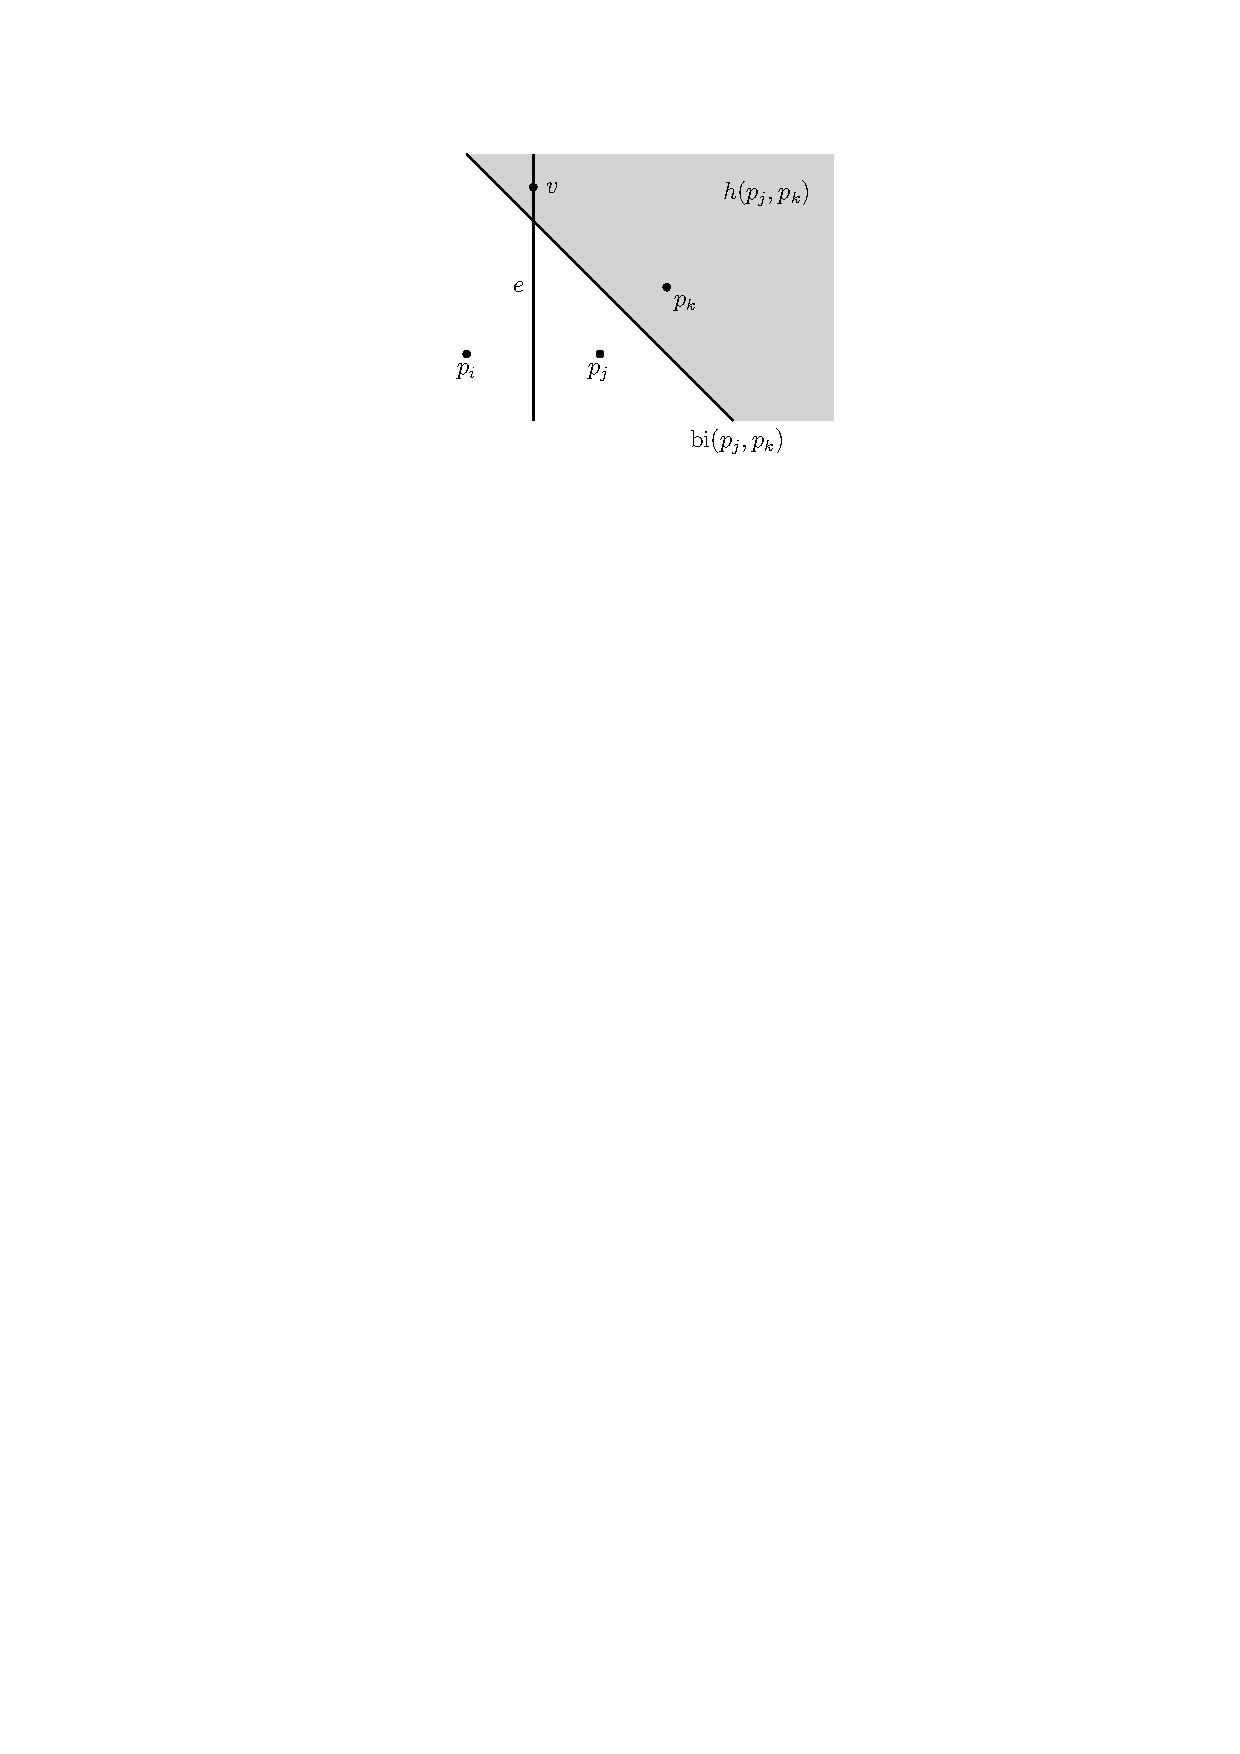
\includegraphics[scale=0.8]{diagram_is_connected} %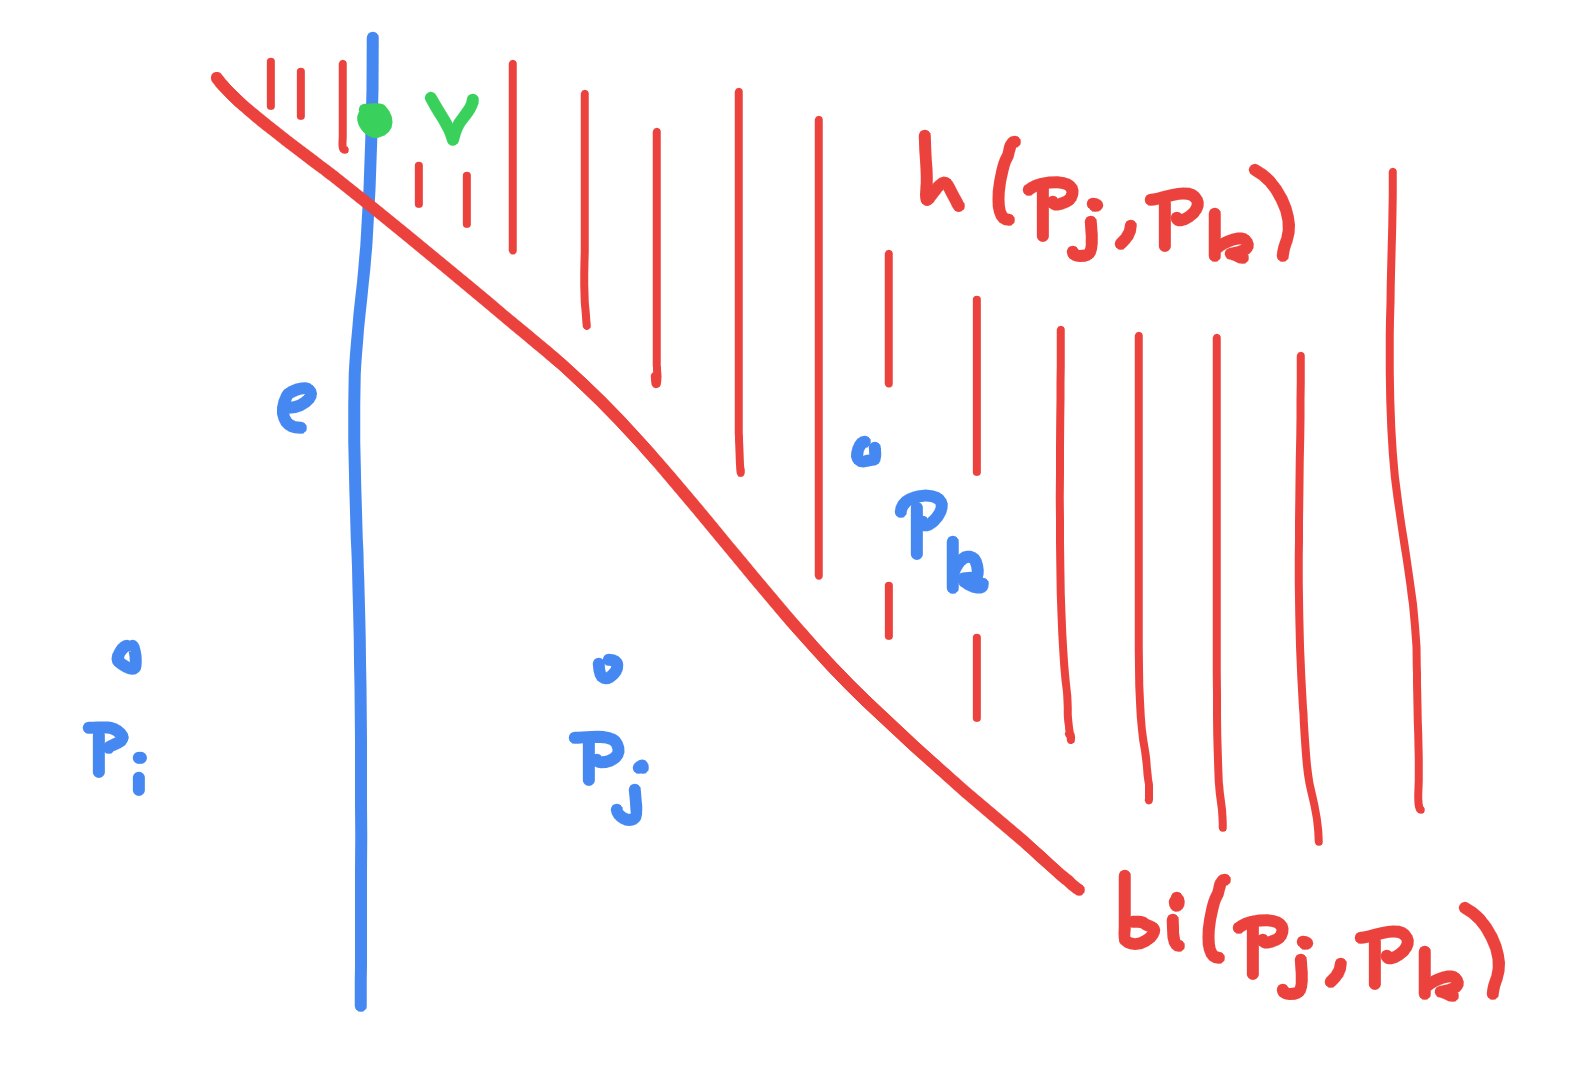
\includegraphics[scale=0.22]{temp-fig-4}
\]
We have that $v \in \partial\mathcal{V}(p_j)$ by definition of $e$. Now note that
\[
    \partial \mathcal{V}(p_j) = \partial \para{\bigcap_{a \ne j} h(p_j, p_a)} \subset^{\footnotemark} \bigcup_{a \ne j} \partial h(p_j, p_a) = \bigcup_{a \ne j} \bi(p_j, p_a).
\]
\footnotetext{Here we used that $\partial(A \cap B) \subset \partial A \cup \partial B$, a proof is here: \url{https://proofwiki.org/wiki/Boundary_of_Intersection_is_Subset_of_Union_of_Boundaries} \todo{Remove this footnote and add the result to some topology appendix}}As $v \in h(p_k, p_j)$ we have that $\dist(v, p_k) < \dist(v, p_j)$, hence $v \not\in \bi(p_j, p_k)$, so $v \not\in \partial{V}(v_j)$ by the above characterization of $\partial \mathcal{V}(p_j)$.
This is a contradiction, so $e$ can't be a full line. Now we show that $\VorG(P)$ is connected. Assume for the sake of a contradiction that $\VorG(P)$ is not connected. Then there exists a $\partial \mathcal{V}(p_i)$ which is not path connected. This can only happen if $\partial \mathcal{V}(p_i)$ consists of two parallel lines \todo{Why?}. This contradicts the fact that $\VorG(P)$ contains no lines. Thus $\VorG(P)$ is connected.
\end{proof}

Finally, we show that that the complexity of the vertices and edges is $\mathcal{O}(n)$:
\begin{thm} \label{thm:numberofvertsandedges}
For $n \geq 3$, the number of vertices in $\VorG(P)$ is at most $2n - 5$ and the number of edges is at most $3n - 6$.
\end{thm}
\begin{proof}
If the points in $P$ are collinear, then Theorem \ref{prop:structureofentirevoronoidiagram} implies the claim. Now assume that the points in $P$ are not collinear. As a first preprocessing step, we start by transforming $\VorG(P)$ into an actual plane graph, as some of the edges in $\VorG(P)$ may be half-lines. Let $v_1, \ldots, v_k$ denote the vertices of $\VorG(P)$. Let $p = \tfrac{1}{k}(v_1 + v_2 + \cdots + v_k) \in \R^2$ and let
\[
    r = 1 + \max\curly{\dist(p, v_1), \dist(p, v_2), \ldots, \dist(p, v_k)}.
\]
Then let $B_r(p) \subset \R^2$ denote the open ball with center $p$ and radius $r$. We have that $B_r(p)$ contains every vertex $v_i$ and that every half-line edge $e$ of $\VorG(P)$ intersects $\partial B_r(p)$ exactly once. Now define $v_{\infty} \in \R^2$ as any point in $\R^2 - B_r(p)$ and transform every half-line edge $e$ into a path with finite length by connecting the half-lines to the point $v_{\infty}$. This is possible since $\R^2 - \overline{B_p(r)}$ only contains these half-lines, and every half-line is pointing in a unique direction so we may then transform the half-lines in order by starting with those which are closest to $v_{\infty}$. An example of this construction is given here:
\[
    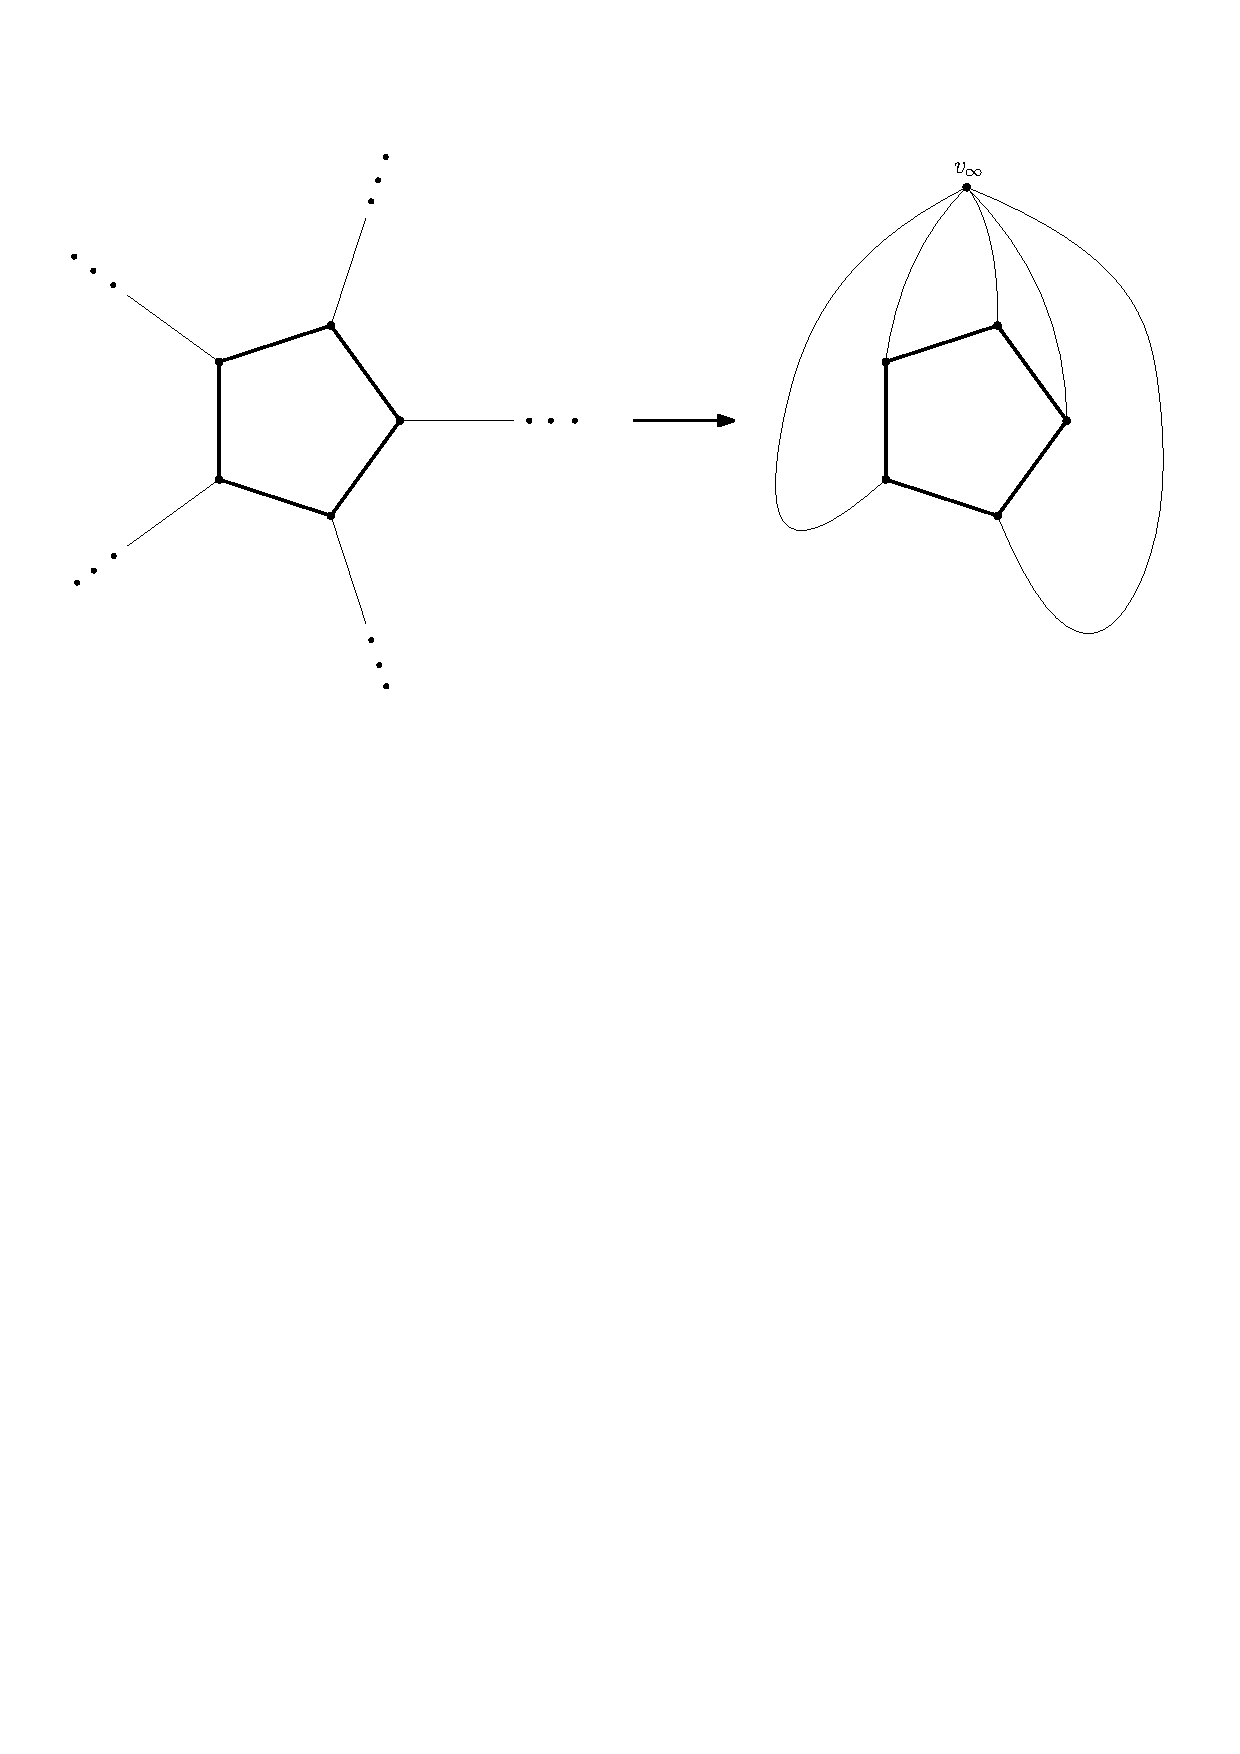
\includegraphics[width=\textwidth]{projective_embedding} % 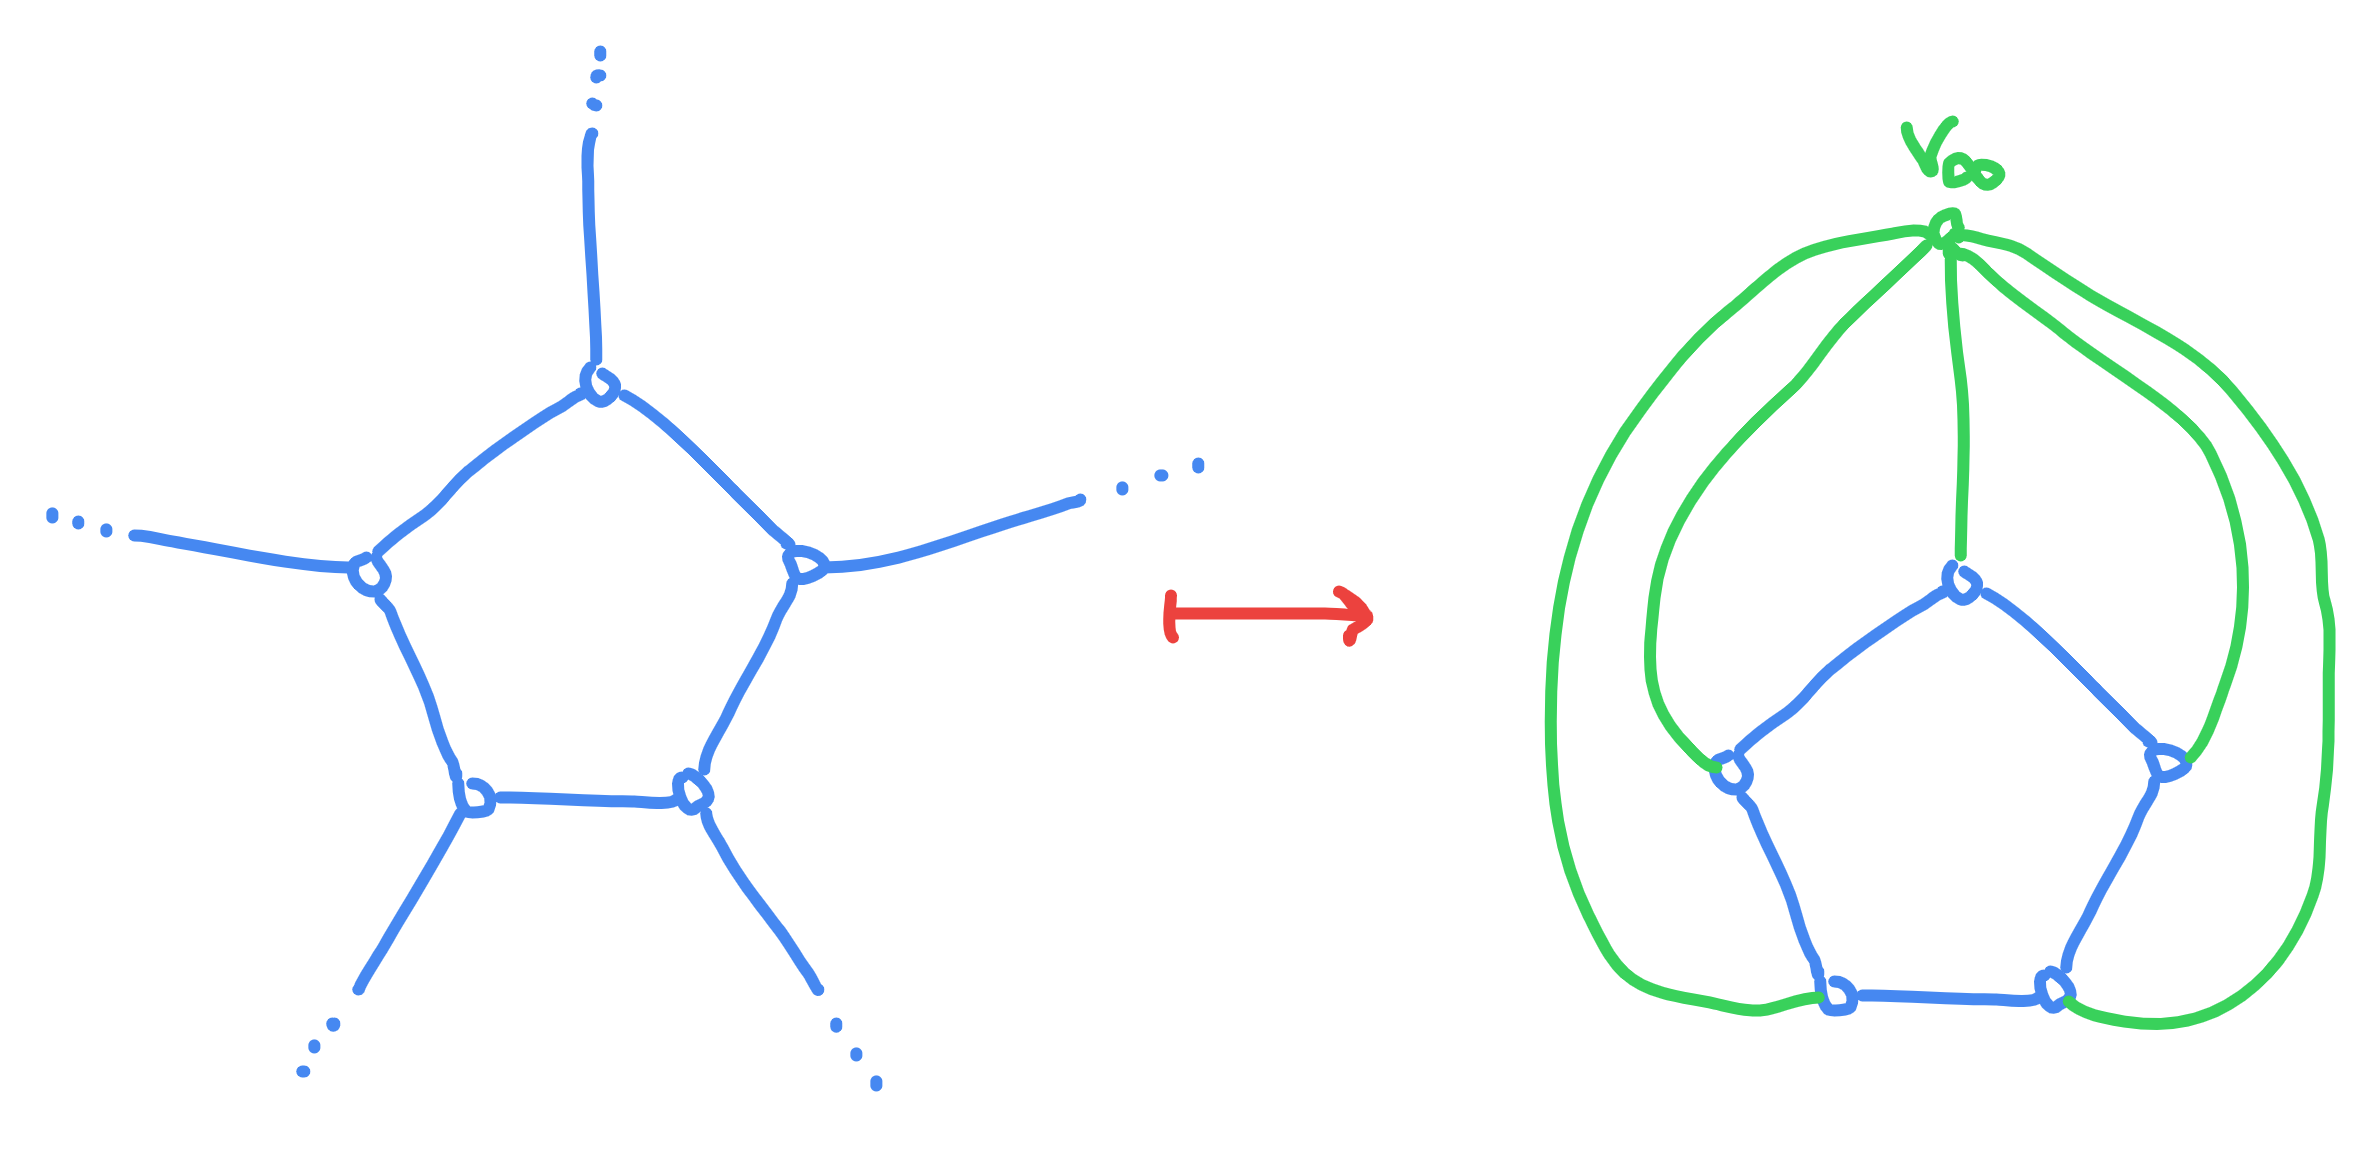
\includegraphics[scale=0.2]{temp-fig-5}
\]
In this way we can turn $\VorG(P)$ into a planar graph. For a planar graph $G$, Euler's formula\footnote{\todo{Add a reference and/or proof of Euler's formula in some topology appendix}} states that
\begin{equation} \label{eq:eulerformulainproof}
    V - E + F = 2,
\end{equation}
where $V$ is the number of vertices, $E$ is the number of edges and $F$ is the number of faces of $G$. Let $n_v$ denote the number of vertices of the original $\VorG(P)$, and let $n_e$ denote the number of edges. In our modification, we only added a single vertex, so by plugging into (\ref{eq:eulerformulainproof}) we obtain the following relationship:
\begin{equation} \label{eq:eulersformulaapplied}
    (n_v + 1) - n_e + n = 2.
\end{equation}
Note that $n$ is the number of faces, since we have a Voronoi cell for each point in $P$. Every vertex $v$ in $G$ has $\deg(v) \geq 3$, otherwise there would be a $\mathcal{V}(p_i)$ which is not convex. This means that
\[
    \sum_{v \in V(G)} \deg(v) \geq 3 \abs{V(G)} = 3(n_v + 1).
\]
Now we want to compute the left side of the above inequality. Given a vertex $v$ we have that $\deg(v)$ counts the number of edges which touch $v$, and in $G$ every edge touches exactly 2 vertices, which gives us that $\sum_{v \in V(G)} \deg(v) = 2 n_e$. Combining these facts, we obtain the inequality:
\begin{equation} \label{ineq:eulersformulacompanion}
    2 n_e \geq 3(n_v + 1).
\end{equation}
Multiplying (\ref{eq:eulersformulaapplied}) by $2$, isolating $2 n_e$ and then applying (\ref{ineq:eulersformulacompanion}) we get:
\begin{align*}
    2 (n_v + 1) - 2 n_e + 2 n = 4
    &\iff 2 n_e = (2 n_v + 1) + 2n - 4 \\
    &\implies 3(n_v + 1) \leq 2 (n_v + 1) + 2n - 4 \\
    &\implies n_v \leq 2n - 5.
\end{align*}
Multiplying (\ref{eq:eulersformulaapplied}) by $3$, isolating $3 (n_v + 1)$ and then applying (\ref{ineq:eulersformulacompanion}) we get:
\begin{align*}
    3 (n_v + 1) - 3 n_e + 3 n = 6
    &\iff 3 (n_v + 1) = 3 n_e - 3n + 6 \\
    &\implies 2 n_e \geq 3n_e - 3n + 6 \\
    &\implies n_e \leq 3n - 6.
\end{align*}
This proves the theorem.
\end{proof}

\section{Characterizing bisectors in the diagram}
We have seen that we have a linear number of vertices and edges $\VorG(P)$, but we have a quadratic number of bisectors $\bi(p_i, p_j)$ of which every edge of $\VorG(P)$ is a subset of, and every vertex in $\VorG(P)$ is an intersection point of two such bisectors. Thus it would be interesting to characterize when a particular bisector is a part of $\VorG(P)$. First, we need a definition:

\begin{defn}[Largest empty circle]
For a $q \in \R^2$ we define $C_P(q)$ to be \emph{the largest empty circle of $q$ with respect to $P$}, which is the largest empty circle with $q$ as its center that does not contain any point of $P$ in its interior. Formally,
\[
    C_P(q) = B_r(q), \quad \text{where} \quad r = \sup\makeset{\lambda \in \R^+}{B_{\lambda}(q) \cap P = \varnothing}.
\]
\end{defn}
\begin{thm} \label{thm:characterizationofbisectors} The bisectors and their intersections are characterized by:
\begin{enumerate}[{(}i{)}]
    \item $q \in \R^2$ is a vertex of $\VorG(P)$ if and only if \[ \abs{\partial C_P(q) \cap P} \geq 3. \]
    \item $\bi(p_i, p_j)$ defines an edge of $\VorG(P)$ if and only if \[ \exists q \in \bi(p_i, p_j) \colon \partial C_P(q) \cap P = \curly{p_i, p_j}. \]
\end{enumerate}
\end{thm}
\begin{proof}
We prove each statement individually:
\begin{enumerate}[{(}i{):}]
    \item ``$\Leftarrow$'': Let $q \in \R^2$ and assume that $\abs{\partial C_P(q) \cap P} \geq 3$. Let $p_i, p_j, p_k$ be three distinct points from $\partial C_P(q) \cap P$. Since $C_P(q) \cap P = \varnothing$ by definition, this means that $q$ is equally close to $p_i, p_j, p_k$ but not closer to any other points in $P$, so $q \in \partial\mathcal{V}(p_i) \cap \partial\mathcal{V}(p_j) \cap \partial\mathcal{V}(p_k) \subset \VorG(P)$, and it is a vertex since it is at an intersection of 3 or more bisectors.

    ``$\Rightarrow$'': Let $q \in \R^2$ be a vertex of $\VorG(P)$. A vertex of $\VorG(P)$ touches at least 3 different edges, and thus touches at least 3 distinct Voronoi cells $\mathcal{V}(p_i), \mathcal{V}(p_j)$ and $\mathcal{V}(p_k)$. So $q \in \partial\mathcal{V}(p_i) \cap \partial\mathcal{V}(p_j) \cap \partial\mathcal{V}(p_k)$. This gives us that
    \[
        \dist(q, p_i) = \dist(q, p_j) = \dist(q, p_k).
    \]
    Denote the above distance by $D$. Now assume for the sake of a contradiction that there exists $p_\alpha \in P$ such that $\dist(q, p_{\alpha}) < D$. Then there are parts of the bisectors $\bi(p_{\alpha}, p_i), \bi(p_{\alpha}, p_j), \bi(p_{\alpha}, p_k)$ contained inside $B_D(q)$, which means that $\mathcal{V}(p_i), \mathcal{V}(p_j), \mathcal{V}(p_k)$ do not all meet at $q$, a contradiction. This means that $C_P(q) \cap P = \varnothing$ and $p_i, p_j, p_k \in \partial C_P(q)$.

    \item ``$\Leftarrow$'': Let $q \in \bi(p_i, p_j)$ such that $\partial C_P(q) \cap P = \curly{p_i, p_j}$. So $C_P(q) \cap P = \varnothing$, which by definition of $C_P(q)$ means that
    \[
        \dist(q, p_i) = \dist(q, p_j) \leq \dist(q, p_k)
    \]
    for all $k$. So $q \in \VorG(P)$ and is either a vertex or an edge. Since $\abs{\partial C_P(q) \cap P} < 3$ part (i) gives us that $q$ is not a vertex, hence it must be an edge, which is a subset of $\bi(p_i, p_j)$. 

    ``$\Rightarrow$'': Let $e \subset \bi(p_i, p_j)$ be an edge of $\VorG(P)$. For $q \in e$ we have that $\dist(q, p_i) = \dist(q, p_j)$, and that $q$ touches $\mathcal{V}(p_i)$ and $\mathcal{V}(p_j)$. By applying the same contradiction proof as in (i) ``$\Rightarrow$'' we have that there is no point in $P$ which is closer to $q$ than $p_i$ and $p_j$, thus $\partial C_P(q) \cap P = \curly{p_i, p_j}$.
\end{enumerate}
\end{proof}

% % % % % % % % % % % % % % % % % % % % % % % % % % % % % % % % % % % %
%
% How to store a Voronoi diagram? DCELs
%
% % % % % % % % % % % % % % % % % % % % % % % % % % % % % % % % % % % % 

\section{The DCEL data structure}
We want to write an algorithm to compute the Voronoi diagram, which leads us to a natural question: how do we store Voronoi diagrams on a computer?  We'll need the following geometric data structure:
\begin{defn}[DCEL] \label{defn:dcel}
A \emph{double connected edge list} (DCEL) is a data structure which represents a subdivision of $\R^2$. A DCEL consists of a lists of vertices, faces and edges. For every edge we will have two copies of it, with opposite orientations, so we will refer to each copy as a directed edge and call it a half-edge, so we actually store a list of half-edges. These three structures are represented as follows:
\begin{description}
  \item[\textsf{Vertex}] $v$ -- represents a vertex of the subdivision. Properties:
  \begin{itemize}
    \item $v.\textsf{position} \in \R^2$: Describes the position of $v$.
    \item $v.\textsf{edge} \text{ is a } \textsf{HalfEdge}$: Points to a half-edge which has $v$ as its start vertex.
  \end{itemize}
  \item[\textsf{Face}] $f$ -- represents a face of the subdivision. Properties:
  \begin{itemize}
    \item $f.\textsf{edge} \text{ is a } \textsf{HalfEdge}$: Points to a half-edge which lies on $\partial f$, and which is a part of a cycle of half-edges which goes around $f$ in counterclockwise order.
  \end{itemize}
  \item[\textsf{HalfEdge}] $e$ -- represents a half-edge of the subdivision. Properties:
  \begin{itemize}
    \item $e.\textsf{origin} \text{ is a } \textsf{Vertex}$: Since the half-edge is directed, we have a first and a second vertex in relation to the edge's direction, and this points to the first vertex.
    \item $e.\textsf{twin} \text{ is a } \textsf{HalfEdge}$: Points to the half-edge with the same vertices as $e$, but pointing in the opposite direction.
    \item $e.\textsf{face} \text{ is a } \textsf{Face}$: Points to the face which lies to the left of $e$.
    \item $e.\textsf{next} \text{ is a } \textsf{HalfEdge}$: Around $e.\textsf{face}$ we have a cycle half-edges which is oriented counterclockwise, and given $e$ in this cycle, $e.\textsf{next}$ gives us the next edge.
    \item $e.\textsf{prev} \text{ is a } \textsf{HalfEdge}$: Around $e.\textsf{face}$ we have a cycle half-edges which is oriented counterclockwise, and given $e$ in this cycle, $e.\textsf{prev}$ gives us the previous edge.
  \end{itemize}
\end{description}
\end{defn}

\begin{rmk}
In the CompGeo book the DCEL structure allows a face to have holes, but since Voronoi diagrams and Delaunay triangulations don't have holes in their faces, we have chosen to omit this feature.
\end{rmk}

\begin{ex}
Consider a graph $G$ with 9 vertices and 10 edges embedded into $\R^2$, which is given as the black figure in the following:
\[
    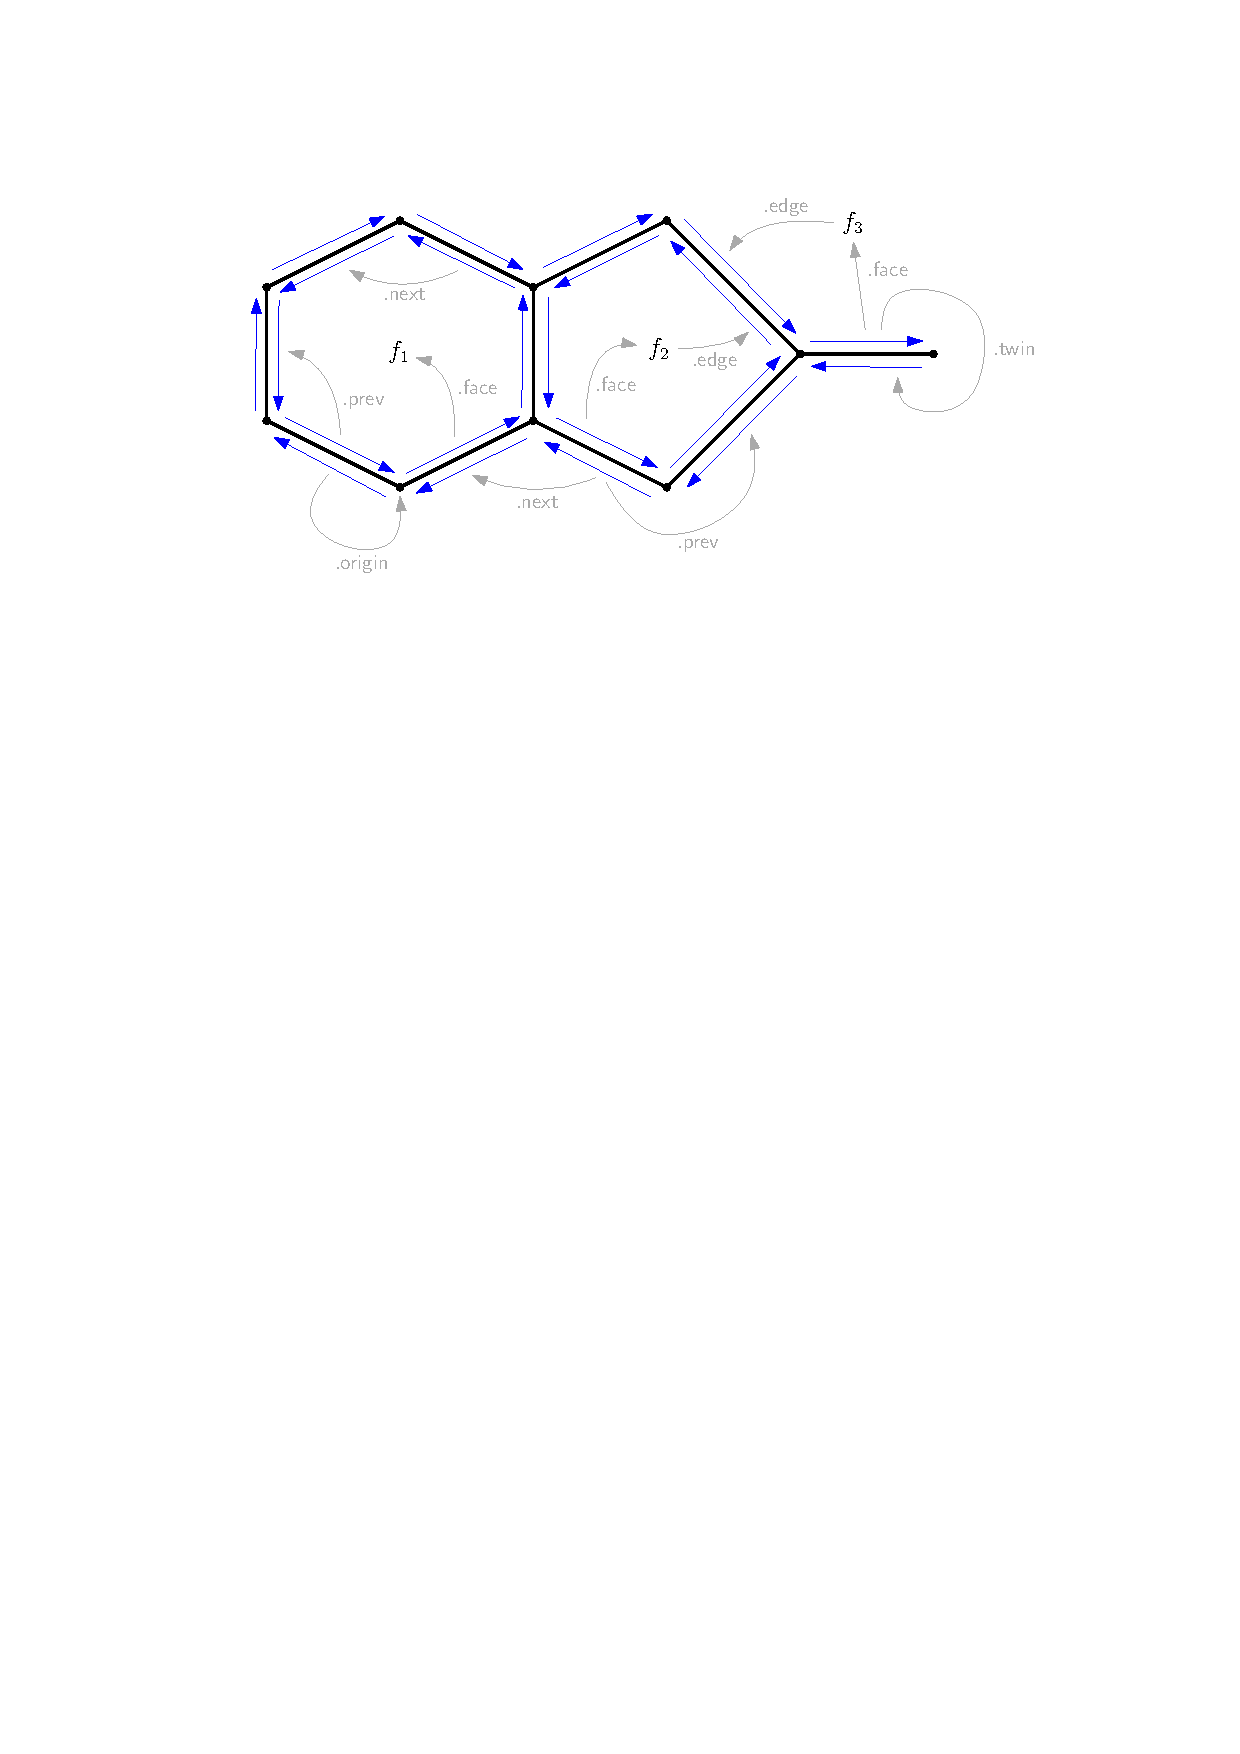
\includegraphics[width=\textwidth]{dcel_example} % 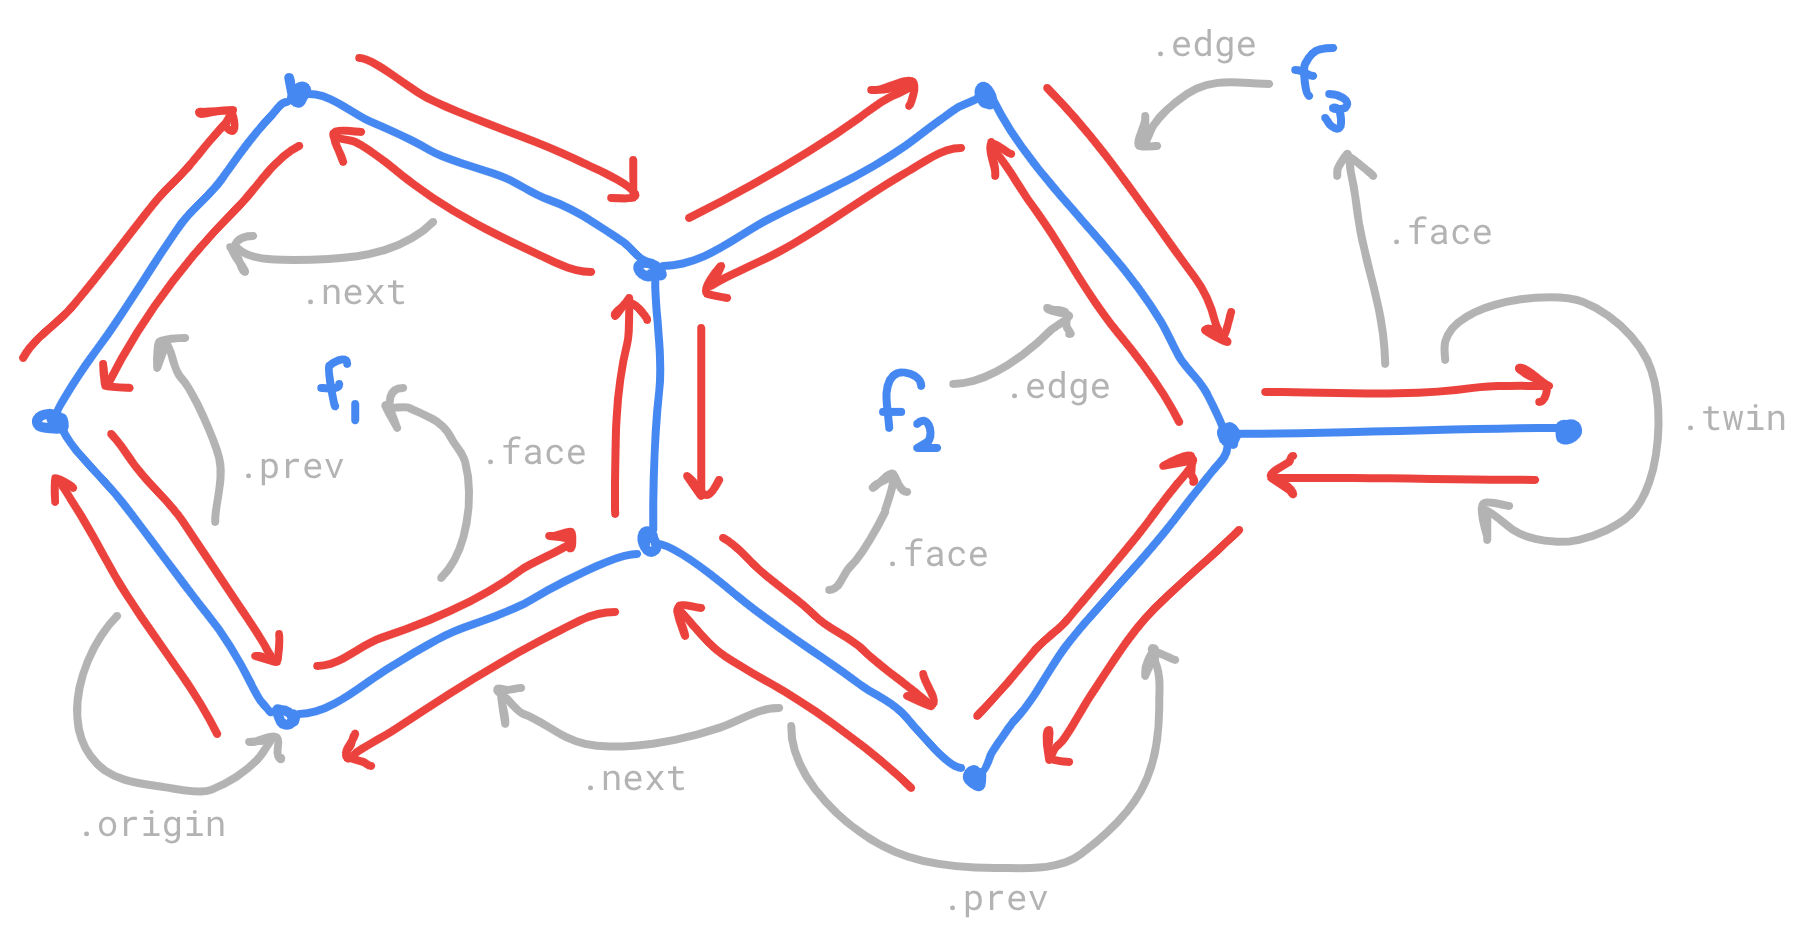
\includegraphics[scale=0.37]{temp-fig-10}
\]
Then this induces a subdivision of $\R^2$ which we represent as a DCEL. The half-edges are given as the blue arrows, the faces as $f_1, f_2, f_3$ and the vertices are the vertices of $G$. Some of the pointers are visible on the figure.

\todo{Make a complete table of everything in the DCEL like the example in the CompGeo book.}
\end{ex}

Note that the DCEL does not support infinite edges, so what we do is put a bounding box $B$ with some padding around the vertices of $\Vor(P)$, and then intersect the infinite edges and faces with the boundary of $B$ and only keep the part inside the bounding box.
\[
    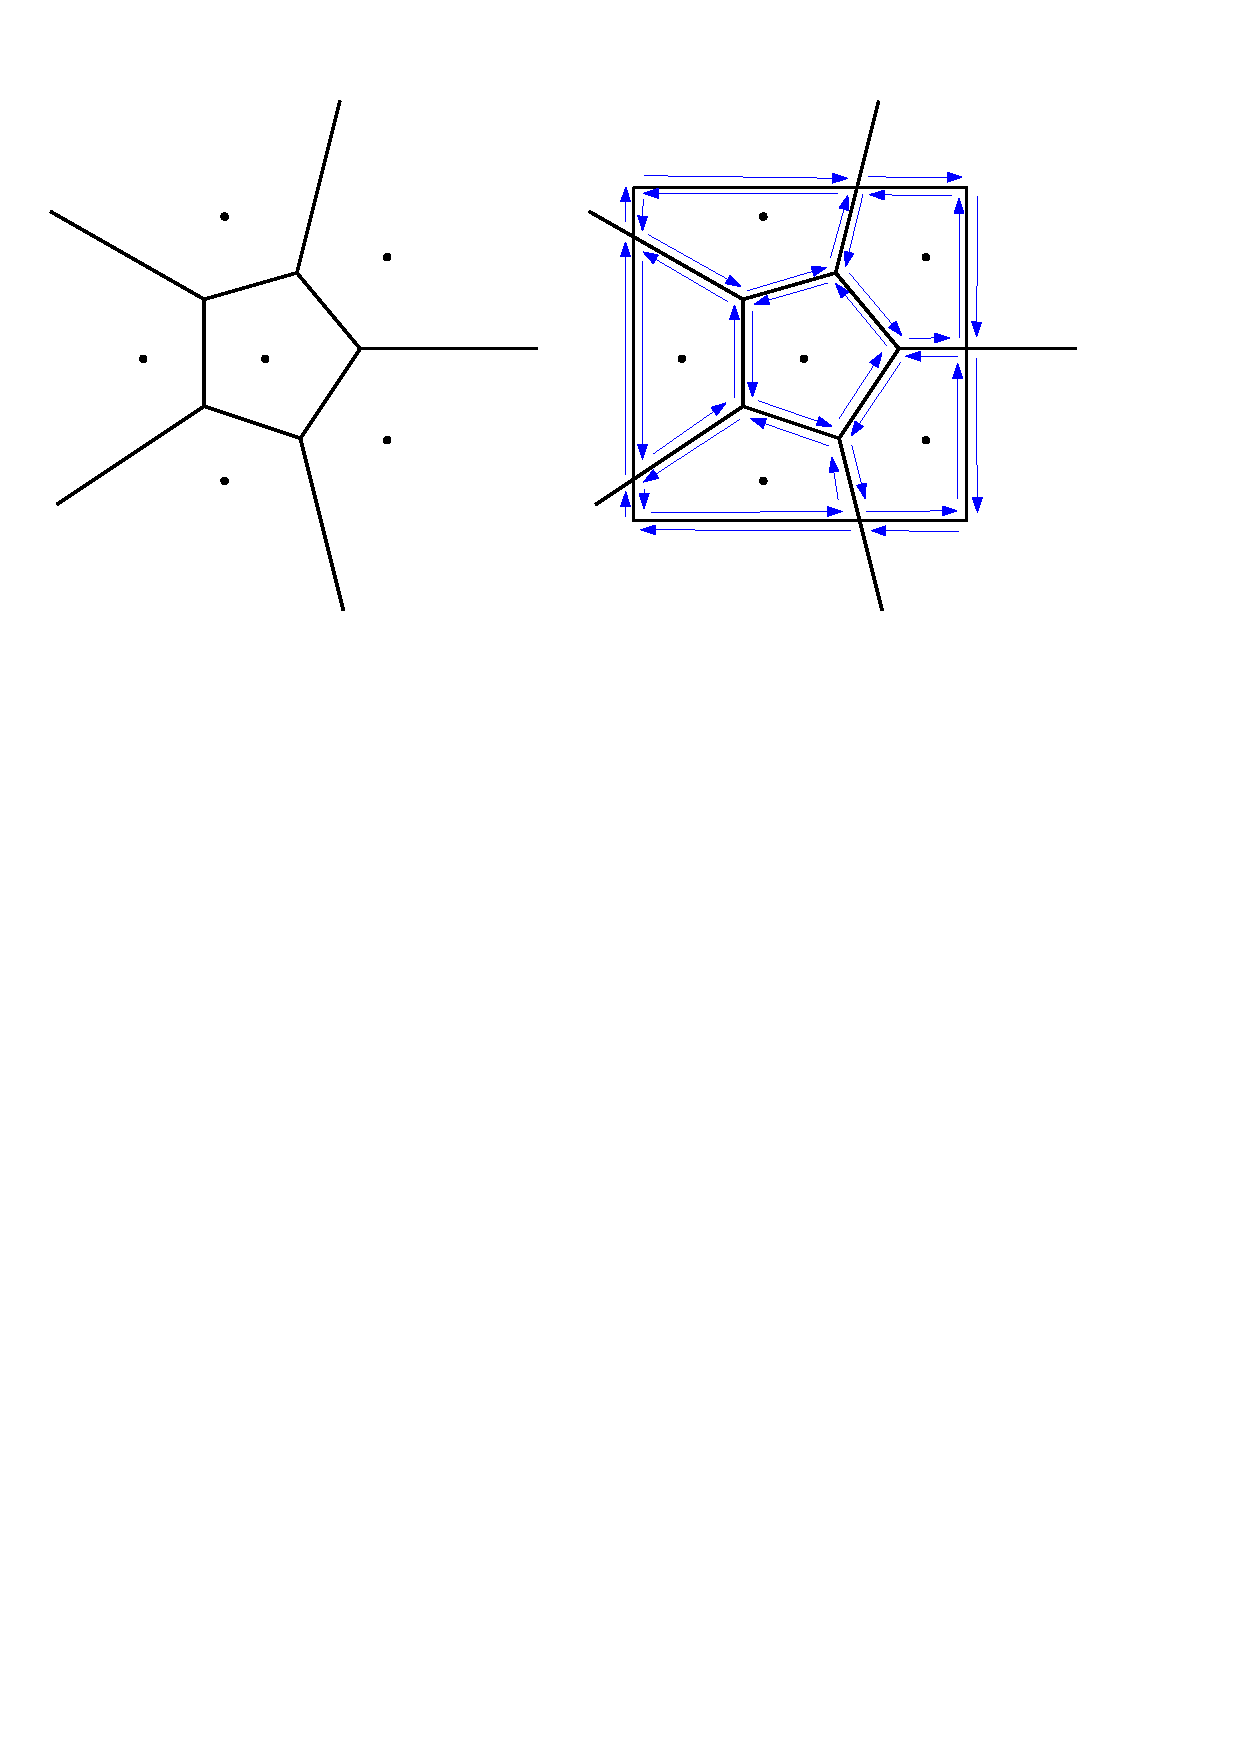
\includegraphics[width=\textwidth]{voronoi_bounding_box} % 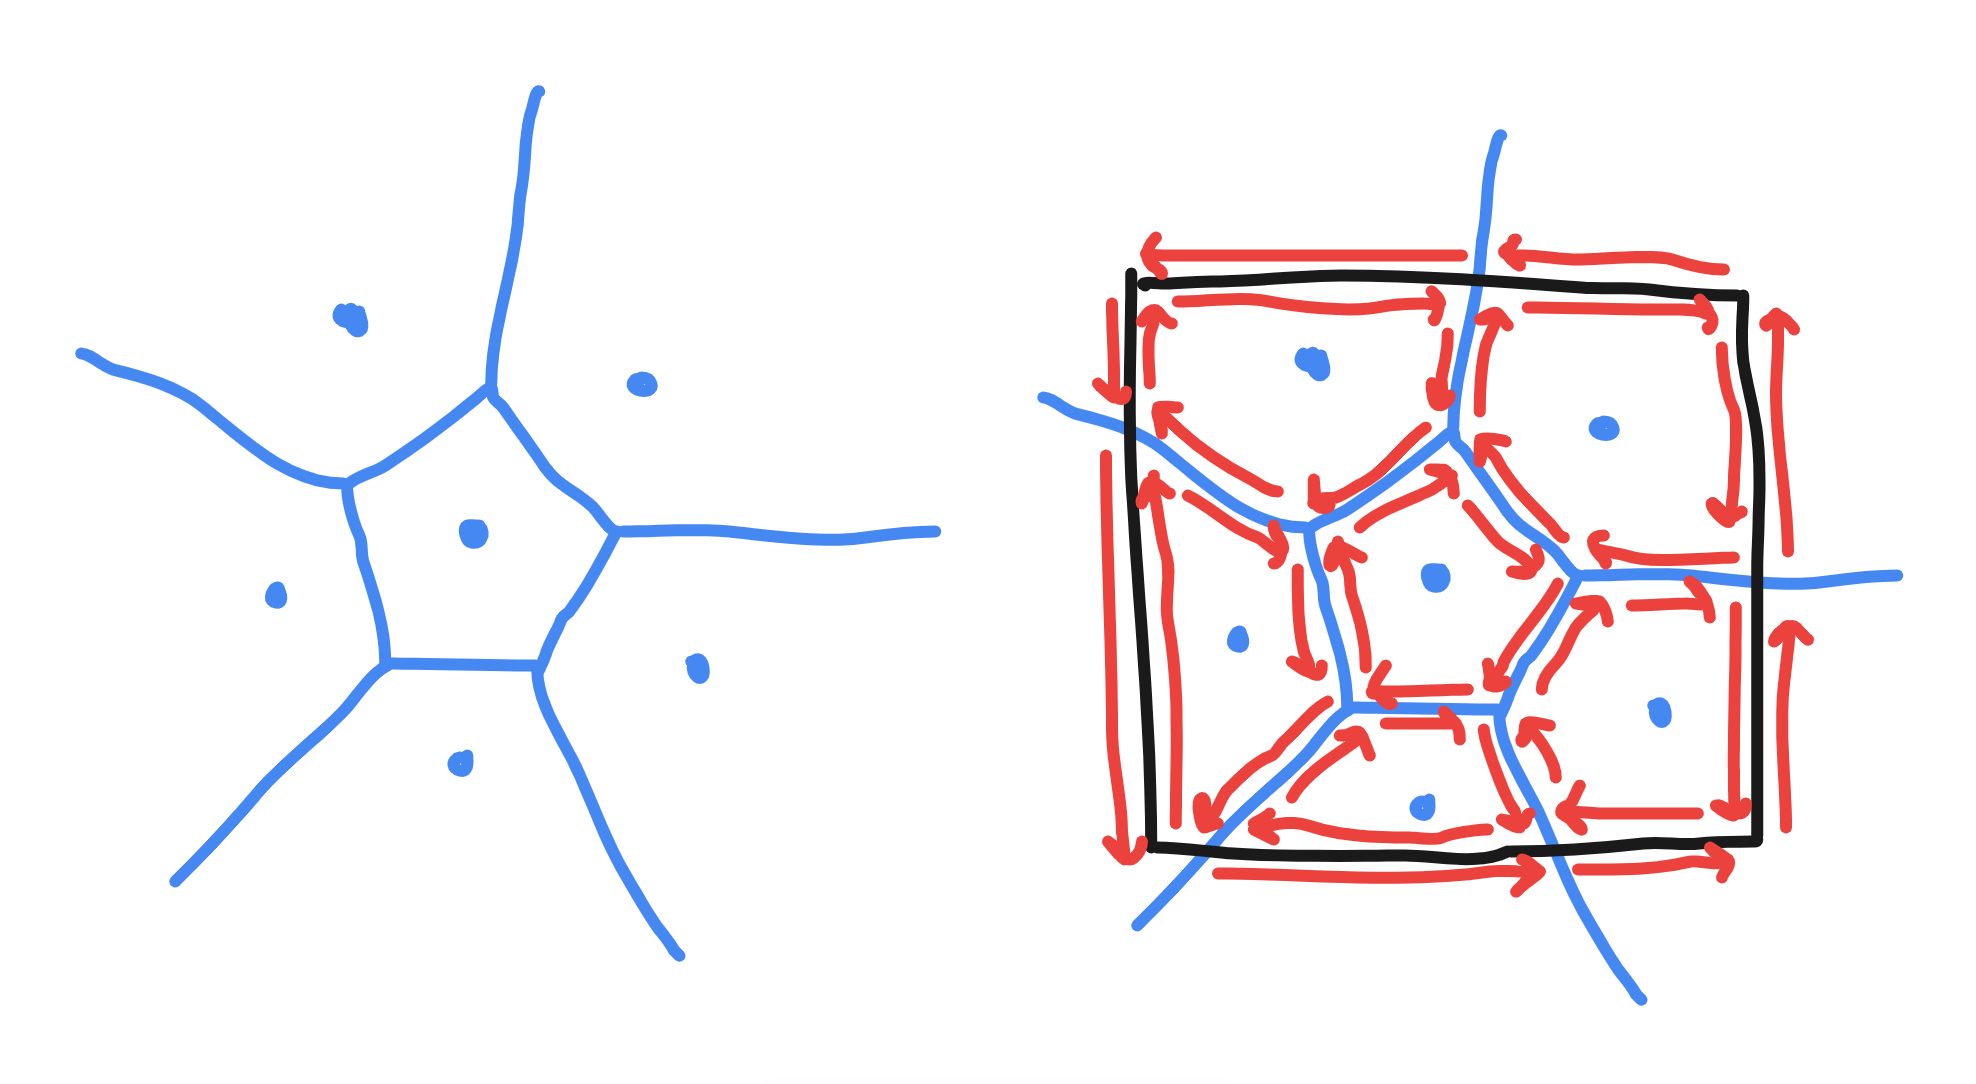
\includegraphics[scale=0.25]{temp-fig-3}
\]
The aim of our algorithms will then be to calculate the DCEL in the right figure.

\begin{rmk} \label{rmk:boxalsohaslinearnumedges}
In practice, we would like to enclose $\Vor(P)$ in a box containing all its vertices in order to be able to represent it as a DCEL $\Delta$. How does intersecting the edges of $\Vor(P)$ with such a bounding box $B$ affect the number of edges?
\[
    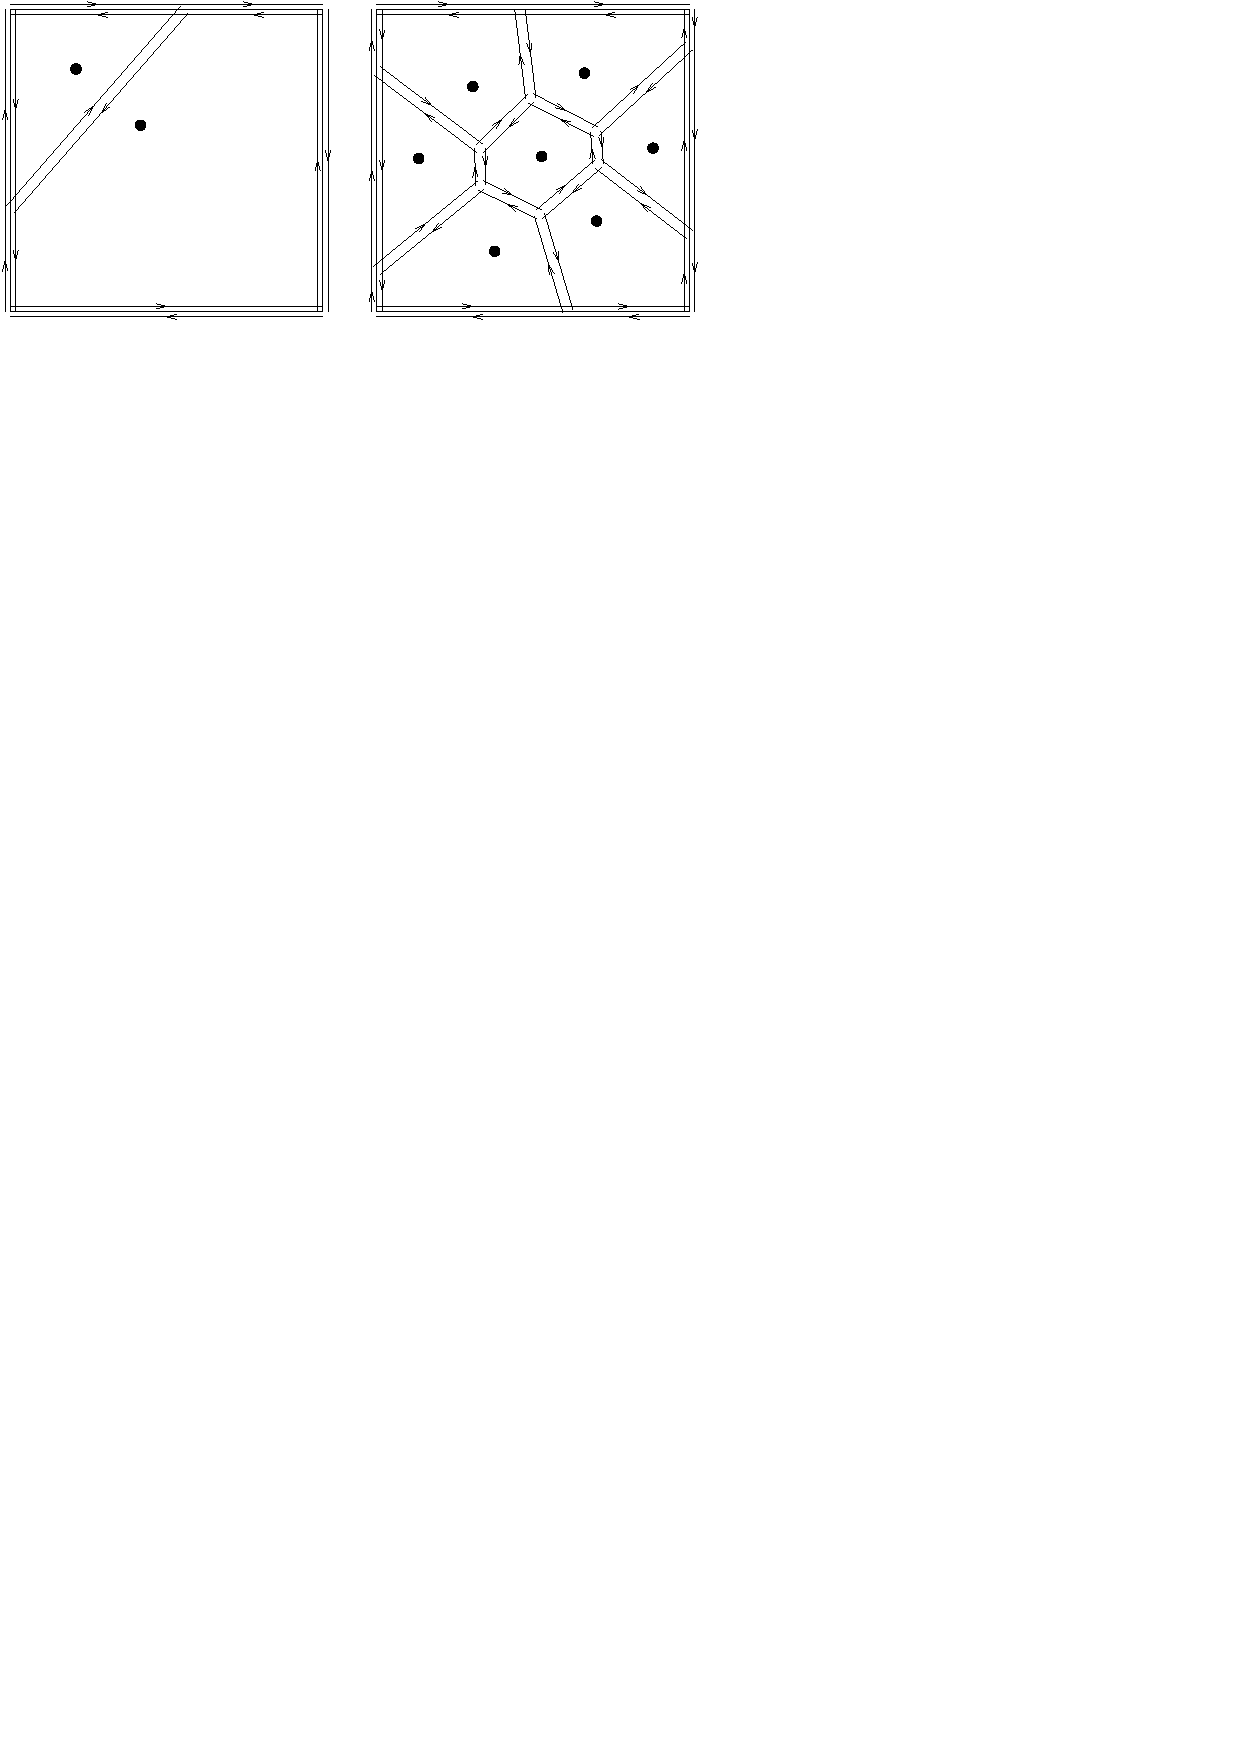
\includegraphics[scale=0.7]{dcel_edges_example}
\]
In the worst case, as depicted on the left figure, 4 new edges may be added to a single unbounded face. In the general case however, as depicted on the right figure, we only introduce between 1-3 edges per face. Thus Theorem \ref{thm:numberofvertsandedges} implies that the complexity is still linear.
%If we intersect $\VorG(P)$ with the bounding box $B$ then $B$ adds at most 2 edges to every cell: The bounded cells inside $B$ stay intact, and for unbounded cells we have two cases. Either a vertex of $B$ is contained in the cell, and then 2 edges will be added, otherwise a single edge is added. Hence in the worst case we add an edge for each point in $P$, and then an edge for each of the 4 corners of $B$, so the DCEL $\Delta$ representing $\Vor(P)$ then has at most
%\[
%    (3n - 6) + (n + 4) = 4n - 2 = \mathcal{O}(n)
%\]
%edges.
\end{rmk}